\subsection{Drone}

På figur \ref{fig:ibd_drone} vises et ibd over drone. Diagrammet viser hvordan alle blokke i dronen er forbundet til main controlleren. Via 3G/GPS modulet sendes og modtages information til og fra drone. Information der modtages fortæller dronen hvor der skal flyves til, hvor der skal tages billeder og om de billeder der tages under flyvning godkendes. Desuden står main controlleren for at styre dronen ud fra data der aflæses fra højde sensor, anti kollision, kompas og GPS. 

\begin{figure}[H]
\centering
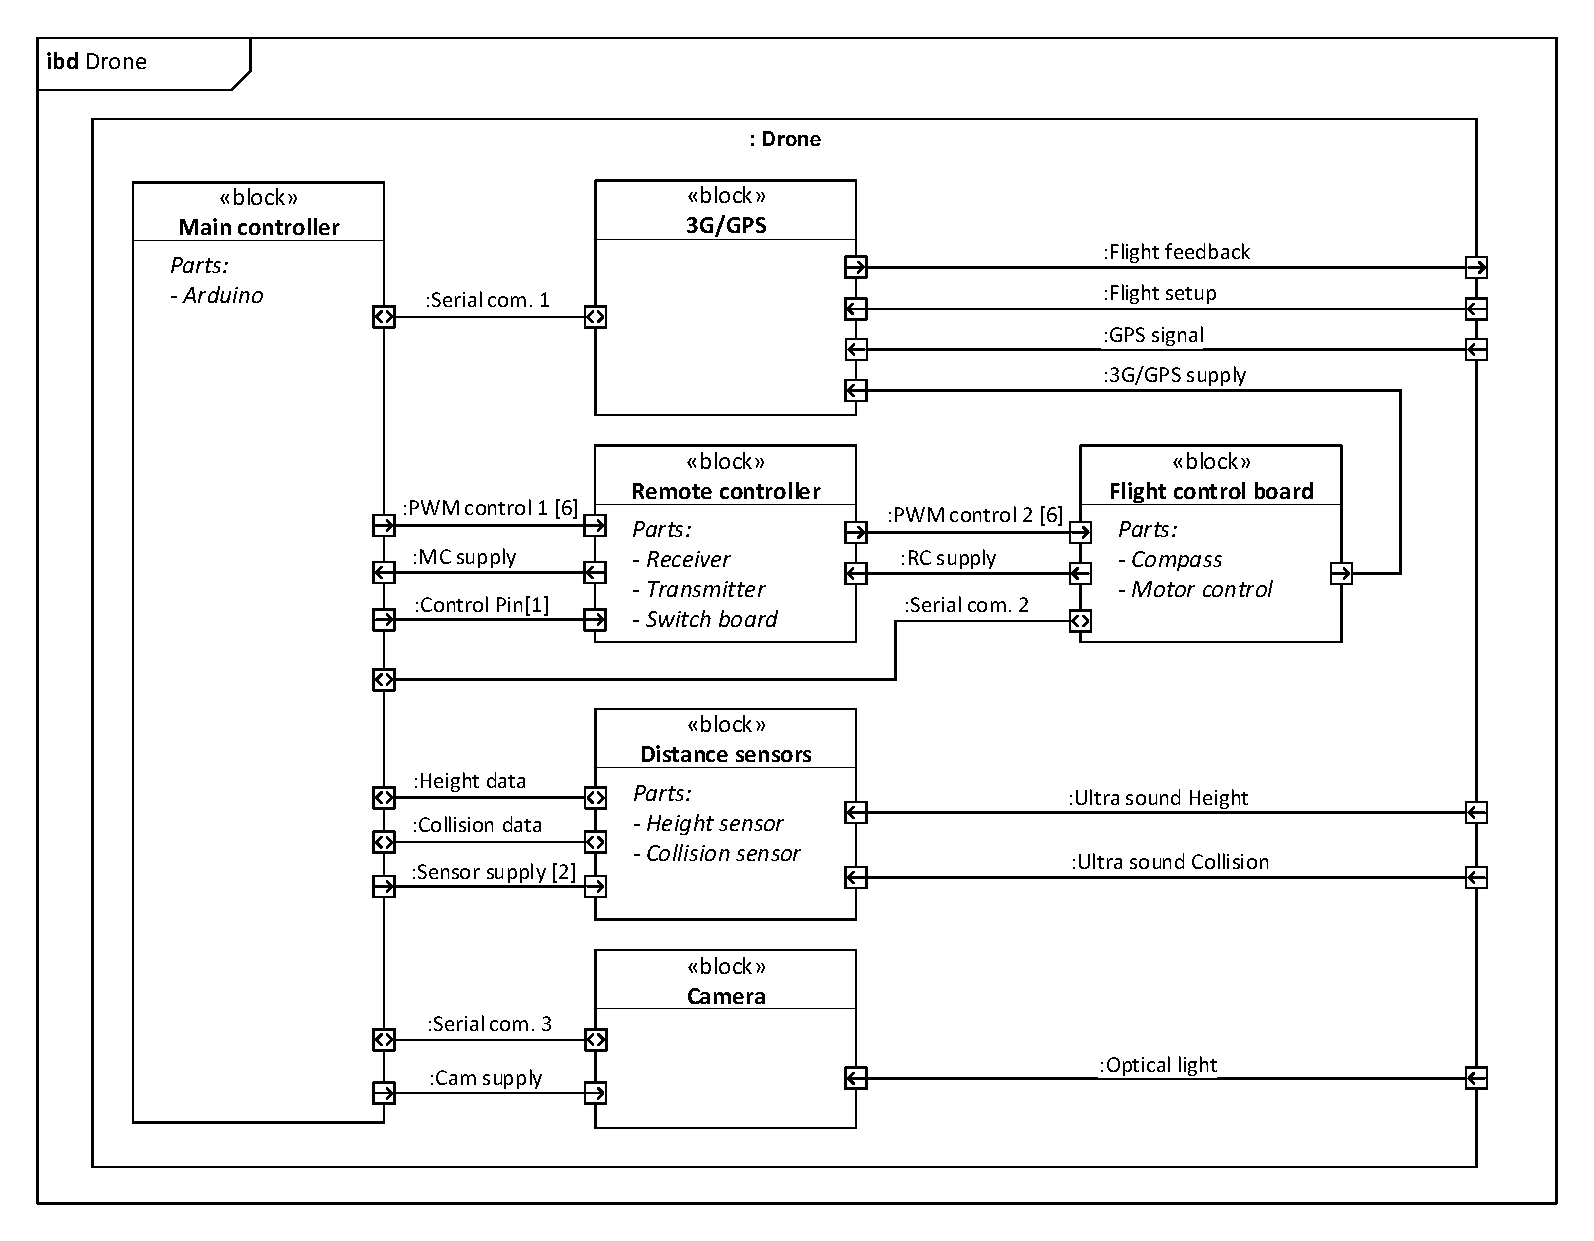
\includegraphics[width=1\textwidth]{Billeder/IBD/ibd2_drone.pdf}
\vspace{-1cm}
\caption{ibd - drone}
\label{fig:ibd_drone}
\end{figure}

\begin{table}[H]
	\centering
		\begin{tabular}{|p{2.6 cm}|p{4.9 cm}|p{2.5 cm}|p{2.5 cm}|}  
		\hline
			\textbf{Signal navn} 	& \textbf{Signal beskrivelse}		& \textbf{Out} 		& \textbf{In}     \\ \hline
			Flight feedback		& Handshake og billeder				& 3G/GPS			& Webapplication	\\ \hline
			Flight setup		& Handshake \& Flyveopsætning  		& Webapplication			& 3G/GPS	\\ \hline
			3G/GPS signal 		& GPS signal	& GPS-satellitter				& 3G/GPS	\\ \hline			
			
			Serial com. 1		& RX / TX signal. Styrer 3G modul. 	& Main controller 	& 3G/GPS    \\ \hline
			3G/GPS supply 		& 3.2 - 4.2 V DC						& Main controller	& 3G/GPS	\\ \hline
			Height data.		& Trigger \& echo signal der indikerer afstanden. 	& Main controller.	& Distance sensors.	\\ \hline
			Kollision data.		& Trigger \& echo signal der indikerer afstanden. 	& Main controller.	& Distance sensors.  \\ \hline
			Sensor supply [2]	& 5V DC forsyning.	& Main controller. & Distance sensors.	\\ \hline
			Serial com. 2		& RX / TX signal. Aflæser data fra kompas & Main controller				& 	\\ \hline 
			PWM control [6]		& 50 Hz 6 kanals signal. Duty cycle 5-10\%. Periode på 20ms	& Main controller.				& Flight control board.	\\ \hline
			Serial com. 3		& RX / TX signal. Styrer kamera	& Main controller	& Camera	\\ \hline
			Cam supply			& 5V DC forsyning. 	& Main controller	& Camera	\\ \hline 
		\end{tabular}
	\caption{Forbindelser til: \textbf{ibd} drone}
	\label{tab:ibddrone}
\end{table}

